\documentclass[tikz,border=3pt]{standalone}

\usepackage{amsmath}
\begin{document}
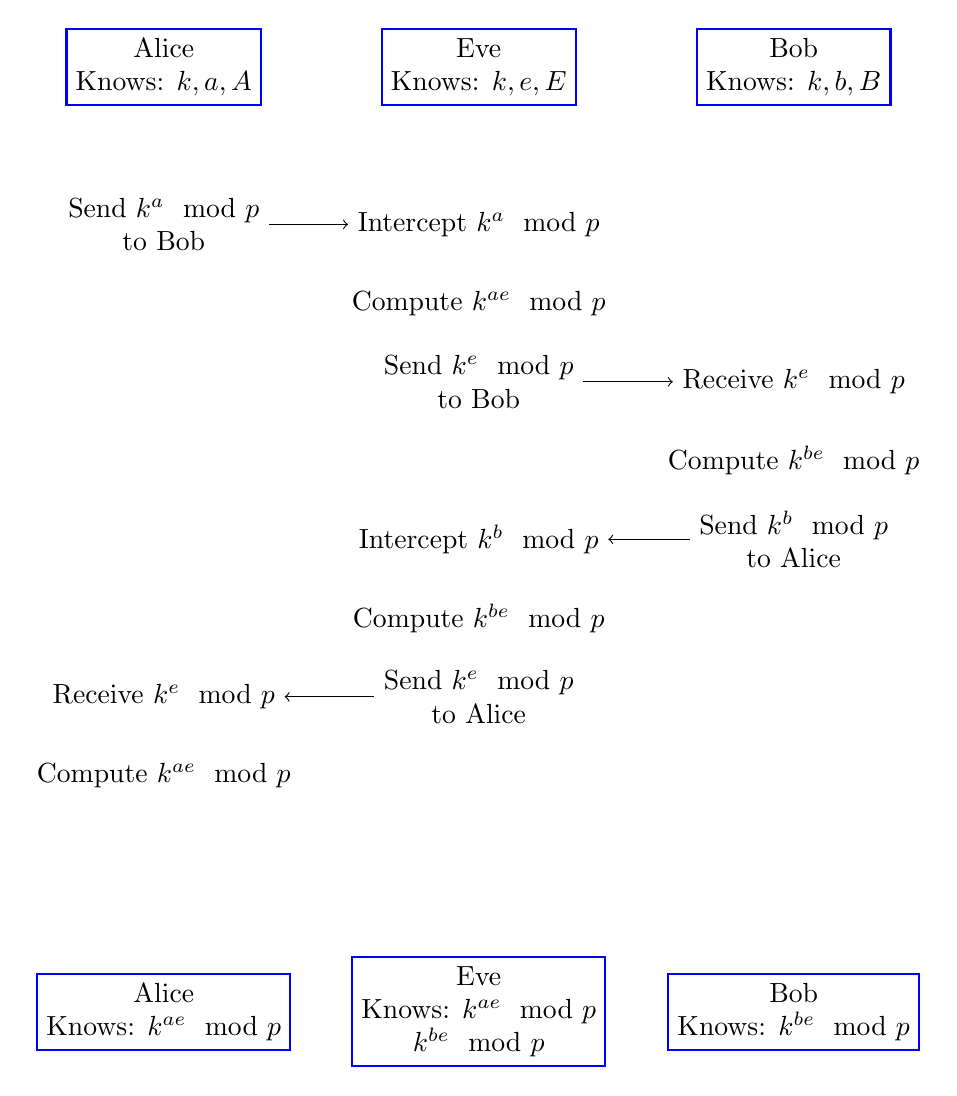
\begin{tikzpicture}[node distance = 4cm]
  \node [rectangle,draw=blue,thick,align=center] (A) {Alice\\Knows: $k,a,A$};
  \node [right of = A, rectangle, draw = blue, thick, align = center] (E) 
  {Eve\\Knows: $k,e,E$};
  \node [right of = E, rectangle, draw = blue, thick, align = center] (B) 
  {Bob\\Knows: $k,b,B$};

  \node [below of = A, node distance = 2cm, align = center] (A2B1) {Send
  $k^a\mod p$\\to Bob};
  \node [right of = A2B1, align = center] (EI1) {Intercept $k^a\mod p$};
  \node [below of = EI1, node distance = 1cm, align = center] (EC1) {Compute
  $k^{ae}\mod p$};
  \draw [->] (A2B1) -- (EI1);

  \node [below of = EC1, node distance = 1cm, align = center] (E2B1) {Send $k^e
  \mod p$\\to Bob};
  \node [right of = E2B1, align = center] (BR1) {Receive $k^e \mod p$};
  \node [below of = BR1, node distance = 1cm, align = center] (BC1) {Compute
  $k^{be}\mod p$};
  \draw [->] (E2B1) -- (BR1);

  \node [below of = BC1, node distance = 1cm, align = center] (B2A1) {Send
  $k^b\mod p$\\to Alice};
  \node [left of = B2A1, align = center] (EI2) {Intercept $k^b\mod p$};
  \node [below of = EI2, node distance = 1cm, align = center] (EC2) {Compute $k^
  {be}\mod p$};
  \draw [->] (B2A1) -- (EI2);

  \node [below of = EC2, node distance = 1cm, align = center] (E2A1) {Send
  $k^e\mod p$\\to Alice};
  \node [left of = E2A1, align = center] (AR1) {Receive $k^e\mod p$};
  \node [below of = AR1, node distance = 1cm, align = center] (AC1) {Compute $k^
  {ae}\mod p$};
  \draw [->] (E2A1) -- (AR1);

  \node [below of = AC1, node distance = 3cm,
  rectangle,draw=blue,thick,align=center] (A2) {Alice\\Knows: $k^{ae}\mod p$};
  \node [right of = A2, rectangle, draw = blue, thick, align = center] (E2) 
  {Eve\\Knows: $k^{ae}\mod p$\\$k^{be}\mod p$};
  \node [right of = E2, rectangle, draw = blue, thick, align = center] (B2) 
  {Bob\\Knows: $k^{be}\mod p$};
\end{tikzpicture}

\end{document}
